% !TEX root = ../thesis.tex

% set counter to n-1:
\setcounter{chapter}{0}

\chapter{Introduction}
A puzzle in the context of video games is conventionally any problem that the player has to solve inside the video game to progress, be it a visual, an auditorial or a dialogue-based problem, and should not be confused with 'Jigsaw puzzles' which are just one possible puzzle type.

Most puzzle games serve as a recreational activity, although they are increasingly used for other purposes, such as for \href{https://www.theguardian.com/technology/2014/jan/25/online-gamers-solving-sciences-biggest-problems}{the gamification of jobs} \cite{TheGuardian}, for \href{https://www.euclidea.xyz}{reframing educational problems as puzzle games} \footnote{\url{https://www.euclidea.xyz}} (also \cite{Lee2014}) or for using them as \href{http://www.gvgai.net}{training grounds for general artificial intelligence} \cite{Perez2014}.

To get a better picture of why people play puzzle games, we conducted a need-finding survey \ref{needfindingq1} where we asked participants, amongst other questions, why they like to play puzzle games. We received the following responses:

\textit{ "to feel smart", "experience aha-moments", "increased spatial reasoning skills", "to get into the state of flow", "because it is fun"}.

Prior literature found similar reasons. In \cite{Kangas2017}, Kangas analyzed the pleasure of puzzles in the context of adventure games and highlights Csikszentmihalyi's work on flow \cite{Csikszentmihalyi}, also referencing flashes of insights and a cycle of suspense and relief as key reasons for player engagement. If the puzzles are too difficult, the player gets frustrated, when the puzzles are too easy, the player gets bored. It is only when the difficulty is just right that the player can get immersed in the challenge and derive pleasure from playing the puzzle. Kangas particularly mentions that puzzles can also be used as part of a broader experience and can help with immersing the player inside the game world by putting them in a state of flow.

 % The correlation between 'difficult for a human' and 'difficult for the program' are still...


%We had a hunch that difficult levels also tend to be fun/interesting.

%We leave the judging of fun to the user and try to optimize for difficult levels based on the guidance of the user. In this way, we exploit both the strengths of the designer and the machine in a mixed-initiative fashion.


\section{Sokoban}

Video games allow for puzzles that cannot easily be played on pen-and-paper (contrary to say Sudoku) since they can have an interactive element to them. A video game could, for example, hide information from the player and only reveal it at a later stage, change the game state while the player tries to solve the level or make it a lot easier to trial-and-error solutions.


One of the arguably first puzzle video games to take advantage of this was Sokoban invented by Hiroyuki Imabayashi in 1981. Inspired by warehouses, in Sokoban, the player controls a person whose job is to push crates/boxes onto storage locations (see image). Since its inception Sokoban has spawned \href{http://www.onlinespiele-sammlung.de/sokoban/list-of-sokoban-games.php}{hundreds of successors} \footnote{\url{http://www.onlinespiele-sammlung.de/sokoban/list-of-sokoban-games.php}} and has inspired countless others. It has also been a popular choice for research, a quick search on Google Scholar reveals roughly 2'040 papers that mention Sokoban at the time of writing, hinting at its popularity.

\begin{figure}[h]
    \centering
    \setlength{\tabcolsep}{0.0130\linewidth}
    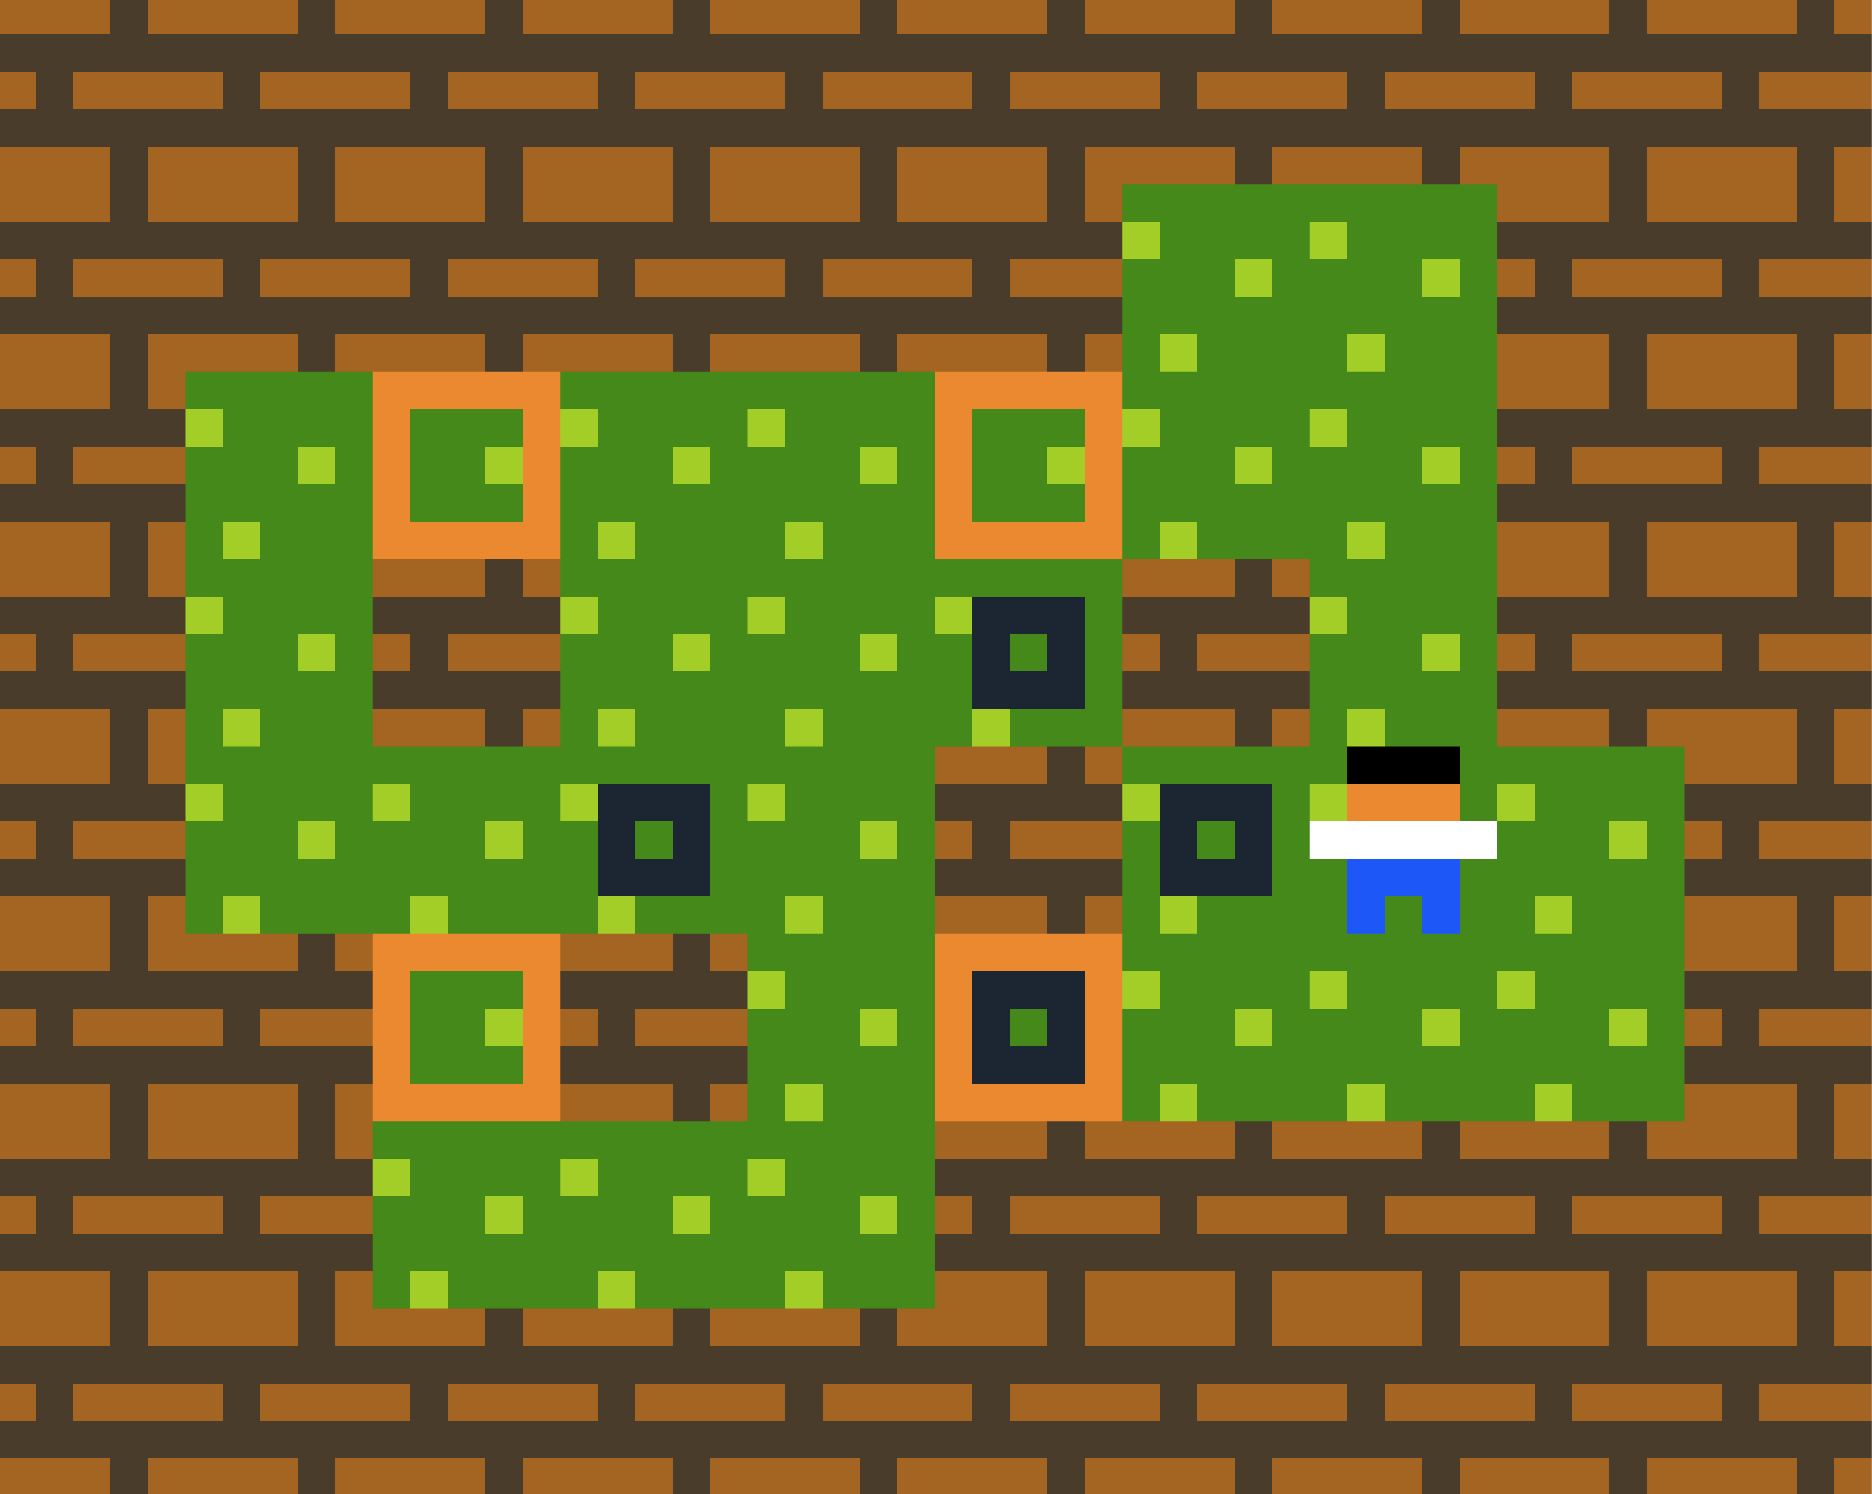
\includegraphics[width=0.487\linewidth]{figures/45minslevel.png}
    
    %\begin{tabular}{@{}cc@{}}
    %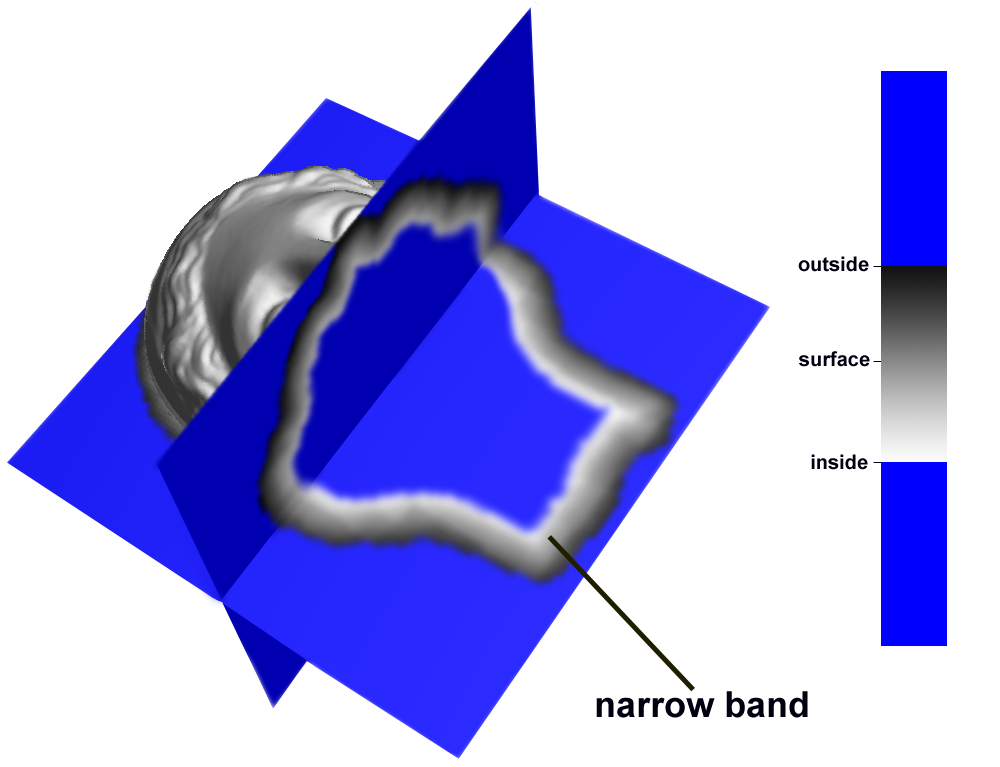
\includegraphics[width=0.487\linewidth]{figures/IgeaNarrowBand}&
    %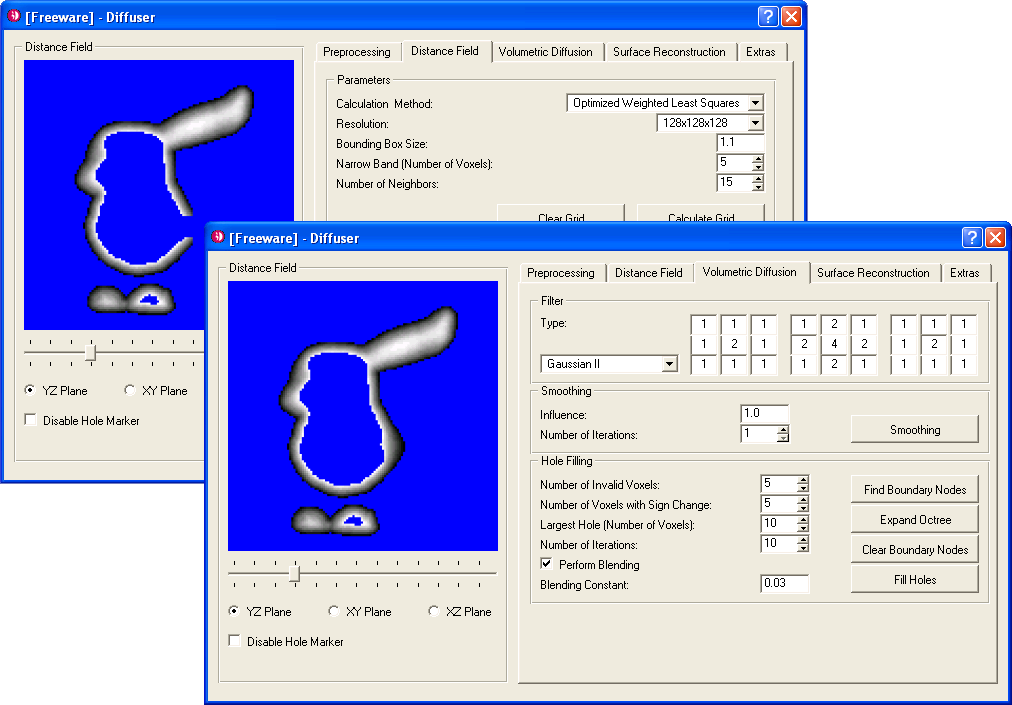
\includegraphics[width=0.487\linewidth]{figures/voldiff_ui}\\
    %(a)&(b)\\
    %\end{tabular}
    \caption[43 Minute Sokoban level]{A Sokoban level taken from \cite{Pelanek2011} %
      \label{fig:43minsfig}}
\end{figure}

Solving a Sokoban level requires much trial-and-error, making it less suited to be played on pen-and-paper. To get a sense of the difficulty, according to \cite{Pelanek2011}, the puzzle in Figure \ref{fig:43minsfig} already takes a median solving time of 43 mins.

For this reason, it only seems natural for designers to correspondingly use tools outside of pen-and-paper when designing Sokoban levels.  
From our need-finding survey \ref{fig:needfindingq3} we know that in practice puzzle designers use a diverse number of approaches and tools. Commercial games have likewise been made with a diverse set of approaches ranging from fully-automated approaches (like Donnantuoni's \href{https://marcosd.itch.io/dispontibus}{Dis Pontibus}\footnote{\url{https://marcosd.itch.io/dispontibus}}) to approaches which are almost exclusively based on pen-and-paper (like Blow's \href{http://the-witness.net}{\url{The Witness}}\footnote{\url{http://the-witness.net}}). Our need-finding survey also, however, showed that designers are open to trying out new interactive methods to add to their design process.

One such tool for designing puzzle games is \href{https://www.puzzlescript.net}{PuzzleScript}\footnote{\url{https://www.puzzlescript.net}} from \href{https://www.increpare.com}{Stephen Lavelle}, a tool all 5 participants from the need-finding interview use, which comes with a level editor (a graphical tool to place the blocks easily) and a run mode (a mode to play-test the designed level). Other than that it does not provide further interactions to create puzzles for puzzle design.


\section{Aim of the study}

This brings us to the aim of this study, which is to develop interactive tools that bring 'genuine value' to the process of puzzle game design, by which interactions are meant, which the designer could not easily attain through direct manipulation (say by using a level editor). For this purpose, we created a mixed-initiative creative interface (MICI) for PuzzleScript called \textit{MixedAim} that allows a tight interaction between the designer and the tool when creating Sokoban-like puzzle games. The reason we choose PuzzleScript was so we could support a broader range of games without giving up much functionality.

\cite{Koch} have shown that computer tools which are both controlled by the human and by the machine, so-called mixed-initiative tools, can be employed successfully to creative tasks like designing moodboards. Moodboards are a collection of images meant to communicate a theme and inspire people who see it. The tool suggests images based on the already designed moodboard, and the user can steer the suggestions using three buttons `more like this', `not this one' and `surprise me'. Similarly, puzzle games are a collection of levels intended to be fun and designed to make the player better at solving them. Our tool MixedAim gives suggestions on how to change a level and allows designers to change the type of suggestions via buttons like `modify this level more' or `change only the walls of this level'. Furthermore, it allows experienced designers to specify their own ways of steering suggestions explicitly.
MixedAim then tries to suggest interesting levels based on these constraints to the user. But what makes a good suggestion? 


\section{Formal theory of fun}
The puzzle games we concern ourselves with are comparable to formal systems, the keyword being \textit{formal} meaning that every state and action inside the game is \textit{well-defined}.
In this analogy, the player starts from a well-defined starting configuration/state (theorem), applies inputs to the puzzle game which lead to well-defined state changes (derivation rules) to achieve a possible well-defined goal configuration (axiom). Usually, puzzle games can have multiple goal states, but they only have a single starting configuration.

In the literature of puzzle games \cite{RulesOfPlay} these well-defined state changes (derivation rules) are called  \textit{operational mechanics}, i.e., the mechanics which are programmed explicitly into the game to make it function (hence the term operational). While playing the game, the player identifies \textit{constituative mechanics} and starts using them in addition to \textit{operational mechanics} to find a solution. For example, in Sokoban, as soon as a crate is pushed next to the right-most wall, there is no way of pushing the crate back from the wall. 

Usually, people concern themselves with formal systems because solving a formal problem (proving a theorem) has useful implications in the real world. For puzzle games, on the other hand, as we have mentioned, it is not very clear why people solve them and which puzzles are more interesting than others.

The best explanation we have found so far comes from Jurgen Schmidhuber's formal theory of creativity, fun, and intrinsic motivation \cite{Schmidhuber}. In a nutshell, the human player is modeled as a reinforcement learner, and the learning process (in this case identifying constituative mechanics and creating a smarter process for solving a level based on these mechanics) is the human player's fun. This also matches with some of the responses of our need-finding study: \textit{"because it is fun.", "experience aha-moments"}.

In more detail, the human player needs to utilizes a certain amount of energy (both mentally and through interaction with the system) to find a goal state. We call this the \textit{subjective difficulty} or correspondingly the \textit{subjective simplicity}. Measuring the \textit{subjective difficulty} quantitatively is difficult since some players stare at a level for a long time before solving it in one go while others start using pen-and-paper to solve a puzzle. It is a lot easier however to measure the energy/the number of operations of a computer program (or as in Schmidhuber's case a reinforcement learner) has to expend in order to find a solution. Schmidhuber also calls this measure the \textit{subjective momentary simplicity} or \textit{compressibility} or \textit{regularity} or \textit{beauty} depending on the problem/context.

Next, while playing a single level, the human discovers constituative mechanics and new strategies of solving levels with these mechanics. This level of discovery is the \textit{subjective interestingness} of a level. Notice that if a player plays the same level over and over the level will start to be less and less interesting to the player. Again quantifying this is very difficult for humans but can be done easily for computer programs (specifically for learning programs). Schmidhuber measures this by subtracting the \textit{subjective difficulty} before solving the level and after solving the level. This way he quantifies how much the program (usually a reinforcement learning program) has learned from playing a level. Schmidhuber also calls this measure \textit{novelty} or \textit{surprise} or \textit{aesthetic reward} or \textit{aesthetic value} or \textit{internal joy} or simply \textbf{fun}, again, depending on the problem/context.

Unfortunately, reinforcement learning algorithms have not been successfully applied to Sokoban, and, to our knowledge, the best Sokoban solvers are not in any shape or form `learning'. Still, we can measure the difficulty of a level by the number of states an algorithm has to explore in order to find a solution.
Since all fun puzzle games feature difficult levels, we had a hunch that difficulty was a useful measure to design fun games. 

Based on this, our final research question becomes: How can interactive tools, specifically tools which focus on providing more difficult level suggestions, aid the user in designing puzzle games?